
\RequirePackage{fix-cm}
%
%\documentclass{svjour3}                     % onecolumn (standard format)
%\documentclass[smallcondensed]{svjour3}     % onecolumn (ditto)
\documentclass[smallextended]{svjour3}       % onecolumn (second format)
%\documentclass[twocolumn]{svjour3}          % twocolumn
%

\RequirePackage{fix-cm}
\smartqed  % flush right qed marks, e.g. at end of proof

\usepackage{cite}
\usepackage{graphicx}
\usepackage{listings}
%\usepackage{pxfonts}
\usepackage{times}
%\usepackage{xspace}
\usepackage{booktabs}
\usepackage{fancybox}
\usepackage{color}
\usepackage{multirow}
\usepackage{array}
\usepackage{tabularx}
\usepackage{url}
\urlstyle{same}
\usepackage{xcolor}
\usepackage{pgfplots}
\usepackage{tikz}
\usepackage{caption}
\usetikzlibrary{shapes,arrows}
\usetikzlibrary{patterns}
\usepackage[numbers]{natbib} % Used to fix formatting issue.
\usepackage{soul} % Needed for wrapping of highlighted text



%\newcommand{\textapprox}{\raisebox{0.5ex}{\texttildelow}}



% Define bar chart colors
%
\definecolor{bblue}{HTML}{4F81BD}
\definecolor{rred}{HTML}{C0504D}
\definecolor{ggreen}{HTML}{9BBB59}
\definecolor{ggrey}{HTML}{707070}
%\definecolor{ppurple}{HTML}{9F4C7C}

% Define flow chart styles
\tikzstyle{decision} = [diamond, draw, fill=blue!20,
    text width=15em, text badly centered, node distance=3cm, inner sep=0pt]
\tikzstyle{block} = [rectangle, draw, fill=blue!20,
    text width=15em, text centered, rounded corners, minimum height=4em]
\tikzstyle{line} = [draw, -latex']


%\makeatletter
%\def\url@foostyle{%
%  \@ifundefined{selectfont}{\def\UrlFont{\sf}}{\def\UrlFont{\small\ttfamily}}}
%\makeatother


\newcommand{\todo}[1]{\textcolor{cyan}{\textbf{[#1]}}}
\newcommand{\emad}[1]{\textcolor{red}{{\it [Emad says: #1]}}}
\newcommand{\dan}[1]{\textcolor{blue}{{\it [Dan says: #1]}}}
\newcommand{\sam}[1]{\textcolor{green}{{\it [Sam says: #1]}}}

\lstset{ %
language=C,                % choose the language of the code
%xleftmargin=100pt,xrightmargin=100pt
basicstyle=\footnotesize,       % the size of the fonts that are used for the code
%numbers=left,                   % where to put the line-numbers
numberstyle=\footnotesize,      % the size of the fonts that are used for the line-numbers
stepnumber=1,                   % the step between two line-numbers. If it is 1 each line will be numbered
numbersep=3pt,                  % how far the line-numbers are from the code
backgroundcolor=\color{white},  % choose the background color. You must add \usepackage{color}
showspaces=false,               % show spaces adding particular underscores
showstringspaces=false,         % underline spaces within strings
showtabs=false,                 % show tabs within strings adding particular underscores
frame=none,           % adds a frame around the code
tabsize=2,          % sets default tabsize to 2 spaces
captionpos=t,           % sets the caption-position to bottom
%captionpos=b,           % sets the caption-position to bottom
breaklines=true,        % sets automatic line breaking
breakatwhitespace=false,    % sets if automatic breaks should only happen at whitespace
escapeinside={\%*}{*)}          % if you want to add a comment within your code
}



\smartqed  % flush right qed marks, e.g. at end of proof
%

% Insert the name of "your journal" with
% \journalname{myjournal}
%
\begin{document}

\title{Examining the Effectiveness of Using Concolic Analysis to Detect Code Clones}


\author{Daniel~E.~Krutz \and
        Emad~Shihab \and
        Samuel~A.~Malachowsky
}

\institute{D. Krutz \at
              Department of Software Engineering, Rochester Institute of Technology, NY USA \\
              \email{dxkvse@rit.edu}           %  \\
           \and
           E. Shihab \at
              % Department of Software Engineering, Rochester Institute of Technology, NY USA \\
               \email{emad.shihab@rit.edu}
 \and
           S. Malachowsky \at
              % Department of Software Engineering, Rochester Institute of Technology, NY USA \\
               \email{samvse@rit.edu}
}

%\date{Received: date / Accepted: date}
% The correct dates will be entered by the editor


\maketitle
\begin{abstract}
During the initial construction and subsequent maintenance of an application, duplication of functionality is common, whether intentional or otherwise. This replicated functionality, known as a code clone, has a diverse set of causes and can have moderate to severe adverse effects on a software project in a variety of ways. A code clone is simply defined as multiple code fragments that produce similar results when provided the same input. While there are an array of powerful clone detection tools, most suffer from a variety of drawbacks including the inability to accurately and reliably detect all four types of clones.

This paper presents a new method for detecting code clones based on concolic analysis, which uses a mixture of concrete and symbolic values to traverse a large and diverse portion of the source code. By performing concolic analysis on the targeted source code and then examining the holistic output for similarities, code clone candidates can be consistently identified. In order to measure the effectiveness of the technique, we performed a case study and found that concolic analysis was able to detect 92\% of known clones in a controlled environment, including a significant number of harder-to-find type-4 clones. Concolic analysis was also able to consistently and effectively locate existing clones in several open source applications with an average precision of 83\% and recall of 93\%, both of which were significantly higher than existing clone detection tools to which they were compared to.

\todo{rewrite abstract based on findings}
\todo{Clean up format based upon new publication}


\keywords{Code Clones \and Concolic Analysis \and Software Engineering}
% \PACS{PACS code1 \and PACS code2 \and more}
% \subclass{MSC code1 \and MSC code2 \and more}
\end{abstract}

\section{Introduction}
Software must continually change in order to keep up with user requirements, enhance its functionality, fix bugs, or repair security vulnerabilities. Prior work has shown that these code changes often results in cloned code for a variety of reasons. In many instances, developers knowingly duplicate functionality across the software system because of laziness or an unwillingness to refactor and retest the modified portion of the application. Careful developers, who know to avoid code clones, may not be aware that identical functionality exists in the system, unintentionally injecting clones into the application~\cite{Duala-Ekoko:2010:CRD:1767751.1767754,Baker:1995:FDN:832303.836911,Kapser:2006:SAC:1133105.1133106,Li:2006:CFC:1128600.1128814}. Whatever the reason, clones continue to be extremely widespread in software development; estimates have shown that clones typically amount to between 5\% and 30\% of an application's source code \cite{Baxter:1998:CDU:850947.853341,Schulze:2010:CCF:1942788.1868310,Kim:2005:ESC:1095430.1081737}.

Many previous works have stated that code clones are undesirable since they often lead to more bugs and make their remediation process more difficult and expensive~\cite{Mondal:2012:ESC:2387358.2387360,Duala-Ekoko:2010:CRD:1767751.1767754,Baker:1995:FDN:832303.836911,Baxter:1998:CDU:850947.853341}. Clones may also substantially raise the maintenance costs associated with an application~\cite{Juergens:2009:CCM:1555001.1555062}, the importance of which is highlighted by the fact that the maintenance phase of a project has been found to encompass between 40\% and 90\% of the totsl cost of a software project~\cite{Shukla:2008:ESM:1342211.1342232,Ducasse:1999:LIA:519621.853389,SMR:SMR225,Ueda:2002:GMS:823457.824039,Boehm:2001:SDR:619059.621640,Erlikh:2000:LLS:612986.613032}. Ultimately, unintentionally making inconsistently applied bug fixes to cloned code across a software system increases the likeliness of further system faults~\cite{Deissenboeck_2010}.

There are four types of code clones generally recognized by the research community. Type-1 clones are the simplest, representing identical code except for variations in whitespace, comments, and layout~\cite{4288192}. Type-2 clones are syntactically similar except for variations in identifiers and types. Type-3 clones are two code segments which are syntactically different due to altered or removed statements. Type-4 clones, the most difficult to detect, are two code segments which have considerable differences syntactically, but produce identical results when executed~\cite{Gold:2010:ICC:1808901.1808916,Dang:2012:XTC:2420950.2421004}.

To assist software practitioners in detecting and managing code clones, clone detection tools have been indispensable in detecting clone-related bugs and even security vulnerabilities in software systems~\cite{Dang:2012:XTC:2420950.2421004}. Of the numerous clone detection tools, most have only been able to detect the simpler clones: type-1, type-2, and type-3. Type-4 clones, the most difficult to detect ~\cite{Yuan:2011:CCM:2114489.2114766,Roy07asurvey}, have, to the best of our knowledge, only two processes able to reliably detect them. MeCC, capable of reliably detecting type-4 clones, suffers from several drawbacks, including the ability to only analyze pre-processed C programs~\cite{Kim:2011:MMC:1985793.1985835}.

In this paper, we examine the effectiveness of using concolic analysis to detect code clones. Concolic analysis combines concrete and symbolic values in order to traverse all possible paths of an application (up to a given length). Traditionally used in software testing to find application faults~\cite{Kim:2012:IAC:2337223.2337373, Kiezun:2013:HSW:2377656.2377662}, concolic analysis forms the basis of a powerful clone detection tool because it only considers the functionality of the source code and not its syntactic properties. Because of this, elements that are challenging for existing clone detection systems such as comments and naming conventions do not affect concolic analysis and its detection of clones.

This research is innovative because, to our knowledge, no previous attempts have been made in using concolic analysis in clone discovery. Any technique which can effectively discover all four types of code clones is important, since, at the present time, so few clone detection processes are able to do so.

Concolic Code Clone Detection (CCCD) is a fully functional tool that uses concolic analysis for clone detection. Concolic analysis is performed on the target application using CREST~\footnote{https://github.com/jburnim/crest/}. First, a Java component uses CTAGS~\footnote{http://ctags.sourceforge.net} to break up the concolic output at the method level. Next, a comparison process uses the developed Levenshtein-distance-based measurement to evaluate the similarity between the concolic output files. Finally, a report displays the detected code clone candidates. This tool, installation instructions, and further details may be found on the project website~\cite{cccd_url} and was published in a previous work~\cite{wcre2013}.


% RQs.
Our study will answer the following research questions:

\textbf{RQ1:}~\emph{What types of clones is concolic analysis effective at detecting?}\\
We find concolic analysis is able to detect all types of clones, in both, a controlled environment and in several open source applications. In a controlled environment using clones identified by previous research, concolic analysis was able to detect 100\% of type-1, type-2, and type-3 clones, and 67\% of type-4 clones.
\todo{update values}

\textbf{RQ2:}~\emph{How does concolic analysis based clone detection compare to other leading clone detection tools?}\\
While several existing methods are very innovative and successful at detecting a variety of code clones, we find that concolic analysis compares very favorably to these tools. Using manually identified clones in several open source systems, concolic analysis consistently discovered clones with a higher rate of precision, recall and F-score when compared to several leading existing clone detection tools. Concolic analysis averaged 83\% for precision, 93\% for recall and an 88\% F-Score while the next leading tool, Nicad, was only able to achieve scores of 66\%, 80\%, and 59\%, respectively.
\todo{update values}


The remainder of the paper is organized as follows. Section~\ref{sec: howconcolicworks} describes how concolic analysis may be used to to detect software clones. Section~\ref{sec: evaluation} evaluates the ability of concolic analysis in identifying clones in relation to existing tools. Section~\ref{sec: discussion} conveys interesting results from the research. Section~\ref{sec: relatedworks} discusses related works in clone detection and concolic analysis. Section~\ref{sec: threats} details some threats to the findings of this work. Section~\ref{sec: conclusion} provides concluding remarks and future research directions for this work.
\todo{update section}


\vspace{-0.08in}
\section{How Concolic Clone Detection Works}
\label{sec: howconcolicworks}

In explaining how concolic code clone detection works, a breakdown of the concept and illustration of it in action is needed. First, we will describe how concolic analysis is performed on two cloned methods. This will include the use of the Levenshtein distance algorithm in measuring the similarity of two sets of concolic output. Next, we will provide a motivating example using a cloned method which has been analyzed by several leading clone detection tools. Finally, we will briefly explain some of the shortcomings of these tools and why concolic analysis was successful in finding the clones.
%\vspace{-0.2in}

\subsection{Concolic Clone Detection Technique}
We will first provide an example of two code clones and then describe how concolic analysis is able to detect these clones. Two type-2 clones are shown in Table~\ref{table:royclones}. These are derived from clones presented by Roy~\emph{et al.}~\cite{Roy:2009:CEC:1530898.1531101}.

%\begin{minipage}{\linewidth}
%\begin{lstlisting}[label=lst:cloneexample1, caption=Type-2 Clone Example \#1, numbers=left]
%void sumProd(int n) {
%	double sum=0.0;
%	double prod =1.0;
%	int i;
%	for (i=1; i<=n; i++){
%		sum=sum + i;
%		prod = prod * i;
%		foo2(sum, prod);
%	}
%}

%\end{lstlisting}
%\end{minipage}

%\begin{minipage}{\linewidth}
%\begin{lstlisting}[label=lst:cloneexample2, caption=Type-2 Clone Example \#2, numbers=left]
%void sumProd2(int n) {
%	int sum=0; //C1
%	int prod =1;
%	int i;
%	for (i=1; i<=n; i++){
%		sum=sum + i;
%		prod = prod * i;
%		foo2(sum, prod);
%	}
%}
%\end{lstlisting}
%\end{minipage}


\noindent
\begin{table*}
\centering
\begin{tabular}{c | c}
\bfseries Code Segment \#1  & \bfseries Code Segment \#2 \\ \hline \hline
\begin{lstlisting}
void sumProd(int n) {
	double sum=0.0;
	double prod =1.0;
	int i;
	for (i=1; i<=n; i++){
		sum=sum + i;
		prod = prod * i;
		foo2(sum, prod);
	}
}
\end{lstlisting}
&
\begin{lstlisting}
void sumProd2(int n) {
	int sum=0; //C1
	int prod =1;
	int i;
	for (i=1; i<=n; i++){
		sum=sum + i;
		prod = prod * i;
		foo2(sum, prod);
	}
}
\end{lstlisting}

\end{tabular}
\caption{An Example of Type-2 clones from Roy~\label{table:royclones}}
\end{table*}

Concolic code clone detection is comprised of two primary phases. The first step is the generation of the concolic output on the target application. This may be done using an existing concolic analysis tool such as CREST~\footnote{http://code.google.com/p/crest/}, Java Path Finder (JPF)~\footnote{http://babelfish.arc.nasa.gov/trac/jpf/}, or CATG~\footnote{https://github.com/ksen007/janala2}.

An abbreviated example segment of concolic output is shown in Listing~\ref{lst:concolicoutput}; the complete output is may be viewed on the project website~\cite{cccd_url}. The generated concolic output represents all executable paths that the software may take, and is broken into several~\emph{path conditions}. These conditions, which are specific to code segments, must be true in order for the application to follow a specified path. For example, if in order to follow a specific path of an~\emph{if} statement a boolean variable must be~\emph{true}, the contingency of the path condition would be that the variable be~\emph{true}. Otherwise, this path will not be traversed~\cite{Sen:2005:CCU:1081706.1081750}.


\begin{minipage}{\linewidth}
\begin{lstlisting}[label=lst:concolicoutput, caption=Example Concolic Output]
										PC#=3
										CONST_3>a_1_SYMINT[2]&&
										CONST_2<=a_1_SYMINT[2]&&
										CONST_1<=a_1_SYMINT[2]

										PC#=2
										CONST_2>a_1_SYMINT[1]&&
										CONST_1<=a_1_SYMINT[1]

										PC#=1
										CONST_1>a_1_SYMINT[2]

\end{lstlisting}
\end{minipage}

In Listing~\ref{lst:concolicoutput}, constant variable types are represented generically by ``CONST'' while the variable type integer is represented by a generic tag ``SYMINT.'' Though not present above, other variable types are represented in a similar fashion in concolic output such as this. Actual variable names do not appear anywhere in the output and are irrelevant to the concolic analysis technique. When comparing the output from the type-2 clones in Table~\ref{table:royclones}, one of the primary differences would be that~\emph{sum} would be defined as a~\emph{double} variable type in the first method while it would be an ~\emph{int} for the second. This would create a small variation in the compared output.
Once this concolic output is created, similar sections of output will be searched for and noted to be code clone candidates. Concolic analysis explores the possible paths that an application can take, with similar execution paths signifying analogous functionality and is thus are indicative of a code clone candidate. Clones in~\emph{dead code} or code that is unreachable via excecution paths will not be analyzed by concolic analysis, and therefore are not discoverable via concolic analysis. To demonstrate this functionality, clones as defined by Roy~\emph{et al.}~\cite{Roy:2009:CEC:1530898.1531101} in Table~\ref{table:royclones} were analyzed using concolic analysis. A portion of the generated concolic output, demonstrated in Table~\ref{table:concolicoutputcomparision}, was then compared for variations. The only difference between the two sets of concolic output is the method name displayed in the first line of each file (an abbreviated listing is shown; full results are available on the project website).


%\begin{figure}[ht!]
%\centering
%\includegraphics[width=110mm,height=70mm]{figures/diffofconcolicoutput.jpg}
%\caption{Diff of Concolic Output}
%\label{fig:concolicoutputcomparision}
%\end{figure}

%\todo{convert this to text}

\noindent
\begin{table*}
\centering
\begin{tabular}{c | c}
\bfseries Concolic Segment \#1  & \bfseries Concolic Segment \#2 \\ \hline \hline
\begin{lstlisting}
sumProd1(a);
PC # 3 = 3
CONST_3 > a_1_SYMINT[2] &&
CONST_2 <= a_1_SYMINT[2] &&
CONST_1 <= a_1_SYMINT[2]
SPC # = 0

PC # = 2
CONST_2 > a_1_SYMINT[1] &&
CONST_1 <= a_1_SYMINT[1]
SPC # = 0

PC # = 1
CONST_1 > a_1_SYMINT[-2]
SPC # = 0
\end{lstlisting}
&
\begin{lstlisting}
sumProd2(a)
PC # = 3
CONST_3 > a_1_SYMINT[2] &&
CONST_2 <= a_1_SYMINT[2] &&
CONST_1 <= a_1_SYMINT[2]
SPC # = 0

PC # = 2
CONST_2 > a_1_SYMINT[1] &&
CONST_1 <= a_1_SYMINT[1]
SPC # = 0

PC # = 1
CONST_1 > a_1_SYMINT[-2]
SPC # = 0
\end{lstlisting}

\end{tabular}
\caption{Diff of Concolic Output~\label{table:concolicoutputcomparision}}
\end{table*}


In order to measure the similarity between sets of the concolic output, the Levenshtein distance measurement is used. This is the minimal number of characters that would need to be replaced to convert one string to another~\cite{Bard:2007:STO:1274531.1274545,Greenhill:2011:LDF:2077692.2077695}. As an example, if the strings ``ABCD'' and ``BCDE'' are measured, the Levenshtein distance would be 2, because ``A'' would need to be removed and ``E'' inserted into the first string to make them identical. This technique was selected for several reasons, but the main motivation related to the impracticality of other string similarity techniques in clone detection using concolic analysis. The Hamming technique, for example, may only be used with strings which are the same length~\cite{Ros:2005:PRR:1086297.1086311, Jain:2012:HES:2324796.2324820}, and concolic output of even two very similar methods rarely yields output of identical length. Another possibility, the longest common subsequence technique, does not account for the substitution of values, only the addition and deletion of characters~\cite{Li:2008:SEA:1593105.1593164}, which also proves problematic.

Because of the relative flexibility of the Levenshtein distance metric, it has proven to be especially well suited for this particular task in clone detection. Due in part to its ability to work with strings of different lengths and its restriction of upper and lower bounds in the calculated distances, normalization is achieved via Equation~\ref{eq:avglevenformula} below. The final Levenshtein score (ALV) is computed by dividing the Levenshtein distance between two files (LD) by the longest string length of the two strings being compared (LSL) and then multiplying by 100.

\begin{equation} \label{eq:avglevenformula}
ALV = (LD/LSL) \times 100
\end{equation}

In order to evaluate the effectiveness of concolic analysis in detecting clones, we created two prototypes. The first was able to analyze source code written in C and utilized CREST in generating the necessary concolic output. The second was created using JPF and examines source code written in Java, though it was not as robust. This Java-based prototype was important because it demonstrated several key concepts, including the assertion that this technique of detecting clones is language agnostic, and that other concolic analysis tools may be used in support of this process. An overview of the entire clone detection technique is shown in Figure~\ref{fig:concolicdiscoveryprocess}.

%\begin{figure}[ht!]
%\centering
%\includegraphics[width=45mm,height=90mm]{figures/ConcolicAnalysis_Process.png}
%\caption{Concolic Analysis}
%\label{fig:concolicdiscoveryprocess}
%\end{figure}

\begin{figure}
\centering
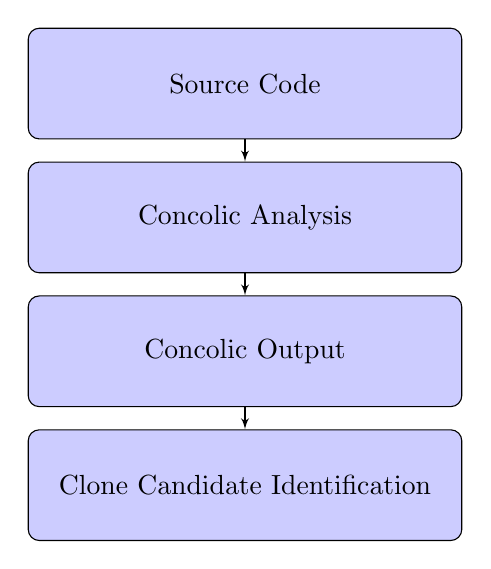
\begin{tikzpicture}[node distance = 1.7cm, auto]
    % Place nodes
    \node [block] (source) {Source Code};
    \node [block, below of=source] (analysis) {Concolic Analysis};
    \node [block, below of=analysis] (output) {Concolic Output};
    \node [block, below of=output] (identification) {Clone Candidate Identification};
    % Draw edges
    \path [line] (source) -- (analysis);
    \path [line] (analysis) -- (output);
    \path [line] (output) -- (identification);

\end{tikzpicture}
\caption{Concolic Analysis} \label{fig:concolicdiscoveryprocess}
\end{figure}

%\vspace{-1.14in}

\subsection{Preliminary Experiments}

A simple comparison was conducted against several leading clone detection tools to further evaluate concolic analysis for code clone detection. This was accomplished using a type-3 clone as defined by Roy~\emph{et al.}~\cite{Roy:2009:CEC:1530898.1531101} and is shown in Table~\ref{table:roy_type3}. The tools used for our analysis are described below.


\todo{add more tools}
\todo{only compare tools that work at the method level?}\dan{It seems like we are often compare tools at different levels, and this makes things apples to oranges}


%\vspace{-0.35in}


\begin{description}
\item~\textbf{Simian:} A text-based tool which uses source transformations and regular expressions to find clones. Simian supports a wide range of languages including Java, C\#, C, C++, ASP, and Ruby. Previous work has demonstrated that this tool finds type-1 and type-2 clones reasonably well, but struggles at discovering the more complicated type-3 and type-4 clones~\cite{simian_URL,Roy:2009:CEC:1530898.1531101}.
\item~\textbf{Nicad:} A text-based hybrid tool that combines the advantages of text and tree-based structural analysis. Clone identification and normalization are conducted using pretty printing and longest common subsequences. Nicad is compatible with C, Java, C\#, and Python and has been found to have the ability to detect type-1, type-2, and type-3 clones, but is known to struggle with type-4 clones~\cite{Roy:2008:NAD:1437898.1438600,Roy:2008:ESF:1447565.1448036,Roy:2009:CEC:1530898.1531101}.
\item~\textbf{CloneDR:} A tree-based clone detection tool which uses hashing and dynamic programming. Annotated parse trees are created using a compiler generator. These trees are then hashed into buckets and compared with one another in the search for clones. This tool is available for numerous languages including C, C++, C\#, Java, and Python and has been found to detect type-1 and type-2 clones very well, type-3 clones with limited effectiveness, and significantly struggles with the identification of type-4 clones~\cite{cloneDR_URL,Baxter:1998:CDU:850947.853341,Rattan20131165,Roy:2009:CEC:1530898.1531101}.
\item~\textbf{MeCC:} Discovers clones by comparing the abstract memory states of an application. A path-sensitive semantic-based path analyzer is first run to estimate the memory states of each method's exit point, then these memory states are then compared to discover clones. Currently only supports preprocessed C programs. The authors of this tool have stated that this tool is able to find all four types of clones with a high rate of accuracy, but there has been a limited amount of other work evaluating this tool ~\cite{Kim:2011:MMC:1985793.1985835,meccURL,kawrykow2011enabling}.
\item~\textbf{Simcad:} A powerful, recently developed clone detection tool derived from a previously created tool called~\emph{simhash} designed to quickly discover exact and near miss clones in large applications. Simcad discovers clones at either the block or function level and is compatible with C, Java, and Python applications. Clone candidates are discovered through the use of three primary phases: pre-processing, detection, and output generation~\cite{6613857}.


\end{description}

%\vspace{-0.50in}



%\begin{table}[thb!]
%\begin{center}
%\caption{Tool Types} % I think these lablels go on top
%    \begin{tabular}{ l | l    }
%%    \toprule
%   \bfseries Tool &\bfseries Technique  \\ \hline \hline
%   \bfseries Nicad & Text   \\ \hline
%\bfseries Simian & Text   \\ \hline
%  \bfseries CloneDR  & Tree   \\ \hline
%\bfseries MeCC & Memory-State   \\ \hline
%\bfseries CCCD & Concolic  \\
%    \end{tabular}
%\end{center}
%\label{table:tooltypes}
%%\vspace{-0.3in}
%\end{table}
%\dan{Should I include this table}



%A version of this example clone was produced in both C and Java.



%\begin{minipage}{\linewidth}
%\begin{lstlisting}[label=lst:sumprod0, caption=Type-3 Clone Example \#3, numbers=left]
%void sumProd1(int n) {
%	  double sum=0.0;
%	  double prod=1.0;
%	  int i;
%	  for (i=1; i<=n; i++){
%		  sum=sum + i;
%		  prod = prod * i;
%		  foo2(sum, prod);
%	  }
%}
%\end{lstlisting}
%\end{minipage}


%\begin{minipage}{\linewidth}
%\begin{lstlisting}[label=lst:sumprod3e, caption=Type-3 Clone Example \#4, numbers=left]
%void sumProd3(int n) {
%	double sum=0.0;
%	double prod =1.0;
%	int i;
%	for (i=1; i<=n; i++){
%		if (i %2 == 0){
%			sum+= i;
%		}
%		prod = prod * i;
%		foo2(sum, prod);
%	}
%}

%\end{lstlisting}
%\end{minipage}
%\sam{This needs a better description of how the type-3 clone plays out}

%\sam{in the following paragraphs, we need to use the same order as listed above (or vise versa)}
%\todo{put these code comparisions side by side}




\noindent
\begin{table*}
\centering
\begin{tabular}{c | c}
\bfseries Code Segment \#1  & \bfseries Code Segment \#2 \\ \hline \hline
\begin{lstlisting}
void sumProd1(int n) {
	  double sum=0.0;
	  double prod=1.0;
	  int i;
	  for (i=1; i<=n; i++){
		  sum=sum + i;
		  prod = prod * i;
		  foo2(sum, prod);
	  }
}
\end{lstlisting}
&
\begin{lstlisting}

void sumProd3(int n) {
	double sum=0.0;
	double prod =1.0;
	int i;
	for (i=1; i<=n; i++){
		if (i %2 == 0){
			sum+= i;
		}
		prod = prod * i;
		foo2(sum, prod);
	}
}
\end{lstlisting}

\end{tabular}
\caption{An Example of Type 3 Clones from Roy~\emph{et al.}~\label{table:roy_type3}}
\end{table*}

\todo{Add in further description of the other tools used and if they could find this clone, and if they could not}

Each of the above detection tools were used, but concolic analysis and MeCC were the only tools able to detect the type-3 clone contained within the example code. CloneDR and Simian were unable to detect this clone because they are tree and text-based clone detection tools; even though the two examined methods are functionally equivalent, they are syntactically different. This is something that these two types of clone detection techniques often struggle with. CodePro is a closed source application and makes no mention of what type of technique it uses for clone detection~\cite{Johnson:2013:WDS:2486788.2486877}, so it is unclear why it was unable to detect this clone. Nicad, essentially a hybrid-based solution, is a text-based detection system which also relies upon the benefits of a tree-based structural analysis and code normalization in order to discover clones~\cite{Roy:2009:CEC:1530898.1531101}. This reliance of the text of the source code likely hindered its ability to find the clone in this example. The size of the functions being examined does not affect the ability of any tools to detect these clones.

MeCC was able to detect this clone since the memory states between the two clones were identical, even though there are syntactic differences between the two compared methods. Concolic analysis was able to detect this clone because it only analyzes the functional nature of the software. The syntactic variations of the two methods which may cause problems for text and syntax-base clone detection tools do not adversely affect the ability of concolic analysis to detect clones. Simcad was also able to identify this clone because it relies on a data clustering algorithm to discover clones, which is not based on the syntactic nature of the code being analyzed~\cite{6613857}.


\section{Evaluation}
\label{sec: evaluation}

\todo{Provide Brief introduction here}
In the following sections, concolic analysis for clone detection will be evaluated individually and against other leading existing clone detection tools.



\subsection{Clone Dataset}
\todo{Describe the datasets that we used}

% Why did we select the data sets that we did
%	Maybe use them all and use a mixture of the results
%	
% Clarifiy some of the questions posed about our dataset
%	The steps used to gather and defines clones (What came first)
% Use the dataset for both parts of the evaluation
% 



% Integrate the discussion of Bellon's work here. Introduce his work and why it is important. Use Bellon as oracle.
% Bellon is used by numerous other research papers \cite{Roy:2008:ESF:1447565.1448036}

%%%% -- End Dataset section

\subsection{Technique Comparisons} %% Give a better Title?

\todo{Provide a better introduction to this}

Our Java-based prototype used Java Path Finder (JPF) to produce the concolic output of the target application. Unfortunately, due to technical limitations of the tool, we were unable to analyze any reasonably sized open source applications using JPF. Of the most profound was its inability perform concolic analysis on several variable types including float, byte, and short, significantly limiting the amount of methods JPF was able to analyze. Without further development, continued use of this tool would have led to inaccurate results since such a large number of methods would have had to been ignored or allowed to produce errors during concolic analysis. Because of this, the Java implementation will only examine proof of concept classes and will not analyze the more complicated Java-based open source applications or similar-sized code bases.

The C-based applications were analyzed by concolic analysis using the Concolic Code Clone Detection (CCCD) tool, published in a previous work by the authors~\cite{wcre2013}. In the previous paper, we demonstrated the ability of concolic analysis to effectively discover all types of code clones in a small, controlled environment. We will build on these results and further compare concolic analysis against several leading existing clone detection tools using clones as defined in previous research by Krawitz~\cite{Kraw2012} and Roy~\emph{et al.}~\cite{Roy:2009:CEC:1530898.1531101}. \\


\textbf{RQ1: \emph{What types of clones is concolic analysis effective at detecting?}}
\todo{update all of this data}

The initial step of evaluating concolic analysis for code clone detection was to evaluate it against 4 clones defined by Krawitz, and 16 by Roy~\emph{et al.}. These 20 defined clones were added to a single Java and C file, and several leading clone detection tools were selected for comparison purposes. For Java, these were CodePro, CloneDR, Simian, Simcad, and Nicad. For C-based applications, Simcad, MeCC, and Nicad were chosen. CodePro and MeCC were only capable of finding clones in Java and C-based applications, respectively. In all examples, the default or recommended settings were used, and the results are shown in Table~\ref{table:singleclasscomparisionexample}. Based on the anemic results early on, Simian and CloneDR were not selected for further evaluation; the remaining tools were subjected to further analysis.

\begin{table}[thb!]
\begin{center}
\caption{Comparison of tools on single class}
\label{table:singleclasscomparisionexample}
\begin{tabular}{r||l|l|l|l|l|l}
%  \hline
\bfseries Application & \bfseries Tool & \bfseries T1 & \bfseries T2 & \bfseries T3 & \bfseries  T4 & \bfseries  Total \\ \hline\hline
  \bfseries Java & CloneDR & 5 & 4 & 0 & 0 & 9 (38\%) \\ \cline{2-7}
   & CodePro &  2 & 3 & 4 & 2 & 11 (46\%) \\ \cline{2-7}
& Simian &  5 & 0 & 0 & 0 & 0 (21\%) \\ \cline{2-7}
& Nicad &  3 & 4 & 4 & 3 & 14 (58\%) \\ \cline{2-7}
& Simcad &  5 & 5 & 6 & 4 & 20 (83\%) \\ \cline{2-7}
 & CCCD  & 5 & 6 & 6 & 6  & 23 (96\%)\\
  \hline
 \bfseries C & CloneDR & 5 & 4 & 0 & 0 & 9 (38\%) \\ \cline{2-7}
   & Simian  & 3 & 2 & 2 & 1 & 8 (33\%) \\ \cline{2-7}
   & MeCC  & 5 & 6 & 6 & 3 & 20 (83\%) \\ \cline{2-7}
& Nicad &  5 & 4 & 4 & 3 & 16 (67\%) \\ \cline{2-7}
& Simcad &  5 & 6 & 7 & 3 & 21 (88\%) \\ \cline{2-7}
 & CCCD  & 5 & 6 & 7 & 4  & 22 (92\%)\\

  \hline
\bfseries Total Possible & & 5 & 6 & 7 & 6 & 24 \\ %\hline

\end{tabular}

\end{center}
%\vspace{-0.3in}
\end{table}

\todo{Describe that the java portion was only a proof of concept}


Within the limited Java implementation, the concolic analysis based technique was able to detect 96\% of all clones, Simcad 83\%, Nicad 58\%, CodePro 46\%, and CloneDR 38\%. The only clone which concolic analysis was unable to detect was a type-3 clone as defined by Roy~\emph{et al.}. JPF, the implementation used by CCCD, was unable to traverse all paths of this method for technical reasons, including its inability to perform analysis on several unsupported variable types (float, byte, and short). This limitation ultimately affects the concolic analysis clone identification process specifically when applied to Java.
\todo{Update above figures}


A similar C file containing the clones of Krawitz and Roy~\emph{et al.} was then examined for clones. Concolic analysis was able to detect 92\% of all clones, Simcad 88\%, MeCC 83\%, and Nicad 67\%. While Simcad, Nicad, and MeCC were all able to discover at least one type-4 clone, none found as many as concolic analysis. All default settings for the clone detection tools were used with complete results being available on the project website~\cite{cccd_url}. In the controlled environment, MeCC, Nicad, and Simcad achieved the best results and were therefore selected for further analysis on larger scale real world applications.
\todo{Update above figures}


The size of the examined functions did not have a significant impact on the ability of any of the examined processes in detecting clones. The only clones that concolic analysis was unable to detect were the type-4 clones as defined by Krawitz. In this clone example, a method has been refactored into two functionally similar methods. Two different concolic paths were generated for these methods, and thus the generated concolic output was not similar, so no clone code candidate was detected.

\textbf{RQ2: \emph{How does concolic analysis based clone detection compare to other leading clone detection tools?}}
\todo{update all of this}

\todo{Talk about and use existing oracles, Bellon etc.....}

In order to compare concolic analysis for clone detection against leading tools in existing systems, we first needed an oracle with predefined clones of all types. Since no known, substantial oracle existed with all four types of clones present, we generated our own. This dataset has been presented and further described in a previous publication~\cite{Krutz_MSR}. To create this oracle, we first selected several open source applications- specifically Apache 2.2.14, Python 2.5.1, and PostgreSQL 8.5 primarily because they had already been used in previous clone detection research~\cite{Kim:2011:MMC:1985793.1985835} and since they are all widely known, open source applications which are publicly available. These applications were selected as-is and had no source code alterations performed. Since we would need to manually verify which methods in the applications were clones, and if so, what type, we then randomly chose 3-6 classes from each application to analyze. The only selection criteria were that the classes needed to contain at least ten methods each, allowing a reasonably sized cross-section for analysis.

Even though only a subset of each application was analyzed, every method would be compared to each other. Because of this, the number of potential clones to be analysed was exponentially large. Within the three applications, there were a total of 45,109 possible clones to verify, a number too large to inspect manually. In order to address this, we selected a statistically significant number of random clone combinations to examine with the goal of having a confidence level of 99\% and a confidence interval of 5. We created an open source tool, CloneInspector~\footnote{https://https://github.com/cloneoracle/CloneInspector/}, to automatically load the selected candidate clone comparisons for manual on-screen analysis. This tool also allowed the user to record whether the comparison was or was not a clone, and, if so, what type of clone it was. Two researchers familiar with code clones independently completed the analysis and any discrepancies with the findings were discussed until an agreement could be reached. The oracle was created before any clone detection efforts ensued to reduce bias during manual analysis. Full results are available on the project website~\footnote{http://phd.gccis.rit.edu/weile/data/cloneoracle/}.

% Talk about the numbers and types of clones that this oracle identified?

\subsection{Types of Discovered Clones}

Most clone detection tools have a variety of input parameters that can be set before analysis. Typically, these include, but are not limited to, the similarity score used to determine if two compared items represent a clone, and the minimum number of required lines for two segments to be recorded as clones. As expected, more stringent settings lead to less false positives, but also less actual clones being discovered. Conversely, lowering these standards may lead to more clones being found, but an inappropriately high number of false positives. The goal is to find the most appropriate balance, optimizing clones found and false positives.

In order to determine the most appropriate settings to use for each tool, we evaluated each using a variety of size and similarity settings against our created oracle. Evaluation criteria included precision, recall, F-score, accuracy, and the number of different clone types found. A similarity score of 70 with a minimum size of 20 was found to achieve the highest scores for MeCC. Nicad has no size parameters and had the best results with a similarity rating of 50. The only relevant settings for Simcad were language, granularity (block of function), and clone type. All compared clone detection tools were made to search for clones at the function level, since this is the same level at which CCCD discovers clone candidates. Further results may be found in the appendix of the paper.

Each tool's findings (including CCCD) by total of each clone type are presented in Table~\ref{table:ClonesFoundByType}. CCCD found the most total clones, as well the most type-2, type-3, and type-4 clones. None of the tools found a significant number of type-1 clones, which is due to the lack of type-1 clones identified in the oracle. This may be largely attributed to the fact that type-1 clones are the easiest to manually locate, and would have likely been recognized and removed by developers in the source code. Nicad was the only other tool to discover any type-4 clones, finding a single pair, while CCCD found 32.

\begin{table}[thb!]

\begin{center}
\caption{Clones Found by Type}
\label{table:ClonesFoundByType}
\begin{tabular}{r||l|l|l|l|l|l}
%  \hline
\bfseries Tool & \bfseries Source Example & \bfseries T1 & \bfseries T2 & \bfseries T3 & \bfseries T4 & \bfseries Total \\ \hline\hline
%  \bfseries Mecc-4 & \bfseries Sample & 5 & 6 & 6 & 3 & 20/24 (83\%) \\ \cline{2-7}
 % \bfseries Mecc & \bfseries Control & x & x & x & x & x \\ \cline{2-7}
\bfseries Mecc & \bfseries Apache & 1 & 16 & 0 & 0 & 17 \\ \cline{2-7}
& \bfseries P-SQL & 0 & 2 & 0 & 0 & 2 \\ \cline{2-7}
& \bfseries Python& 0 & 6 & 6 & 0 & 12 \\ \cline{2-7}
& \bfseries Total & \bfseries 1  & \bfseries 24   & \bfseries 6  & \bfseries 0  &  \bfseries 31 \\ \cline{2-7}


% \hline \hline
% \bfseries CloneDR-80 & \bfseries Sample & 5 & 4 & 0 & 0 & 9/24 (38\%) \\ \cline{2-7}
% \bfseries CloneDR & \bfseries Control & 6 & 7 & 0 & 0 & 13 \\ \cline{2-7} %CloneDR80
%& \bfseries Apache & 0 & 2 & 0 & 0 & 2 \\ \cline{2-7}
%& \bfseries P-SQL & 0 & 0 & 0 & 0 & 0 \\ \cline{2-7}
%& \bfseries Python& 0 & 0 & 0 & 0 & 0 \\ \cline{2-7}
 \hline \hline
 %\bfseries Simcad & \bfseries Control & x & x & X & X & X \\ \cline{2-7} %CloneDR80
\bfseries Simcad & \bfseries Apache & 0 & 12 & 0 & 0 & 12 \\ \cline{2-7}
& \bfseries P-SQL & 0 & 0 & 0 & 0 & 0 \\ \cline{2-7}
& \bfseries Python& 0 & 5 & 7 & 0 & 12 \\ \cline{2-7}
& \bfseries Total & \bfseries 0  & \bfseries 17   & \bfseries 7  & \bfseries 0  &  \bfseries  24 \\ \cline{2-7}
 \hline \hline
% \bfseries Simian & \bfseries Sample & 3 & 2 & 2 & 1 & 8/24 (33\%) \\ \cline{2-7}
% \bfseries Simian & \bfseries Control & 6 & 3 & 14 & 0 & 23 \\ \cline{2-7}
%& \bfseries Apache & 0 & 1 & 0 & 0 & 1 \\ \cline{2-7}
%& \bfseries P-SQL & 0 & 0 & 0 & 0 & 0 \\ \cline{2-7}
%& \bfseries Python& 0 & 0 & 0 & 0 & 0 \\ \cline{2-7}
 %\hline \hline
% \bfseries Nicad & \bfseries Sample & 5 & 4 & 4 & 3 & 16/24 (67\%) \\ \cline{2-7}
% \bfseries Nicad & \bfseries Control & x & x & x & x & x \\ \cline{2-7}
 \bfseries Nicad & \bfseries Apache & 1 & 16 & 0 & 0 & 17 \\ \cline{2-7}
& \bfseries P-SQL & 0 & 2 & 1 & 1 & 4 \\ \cline{2-7}
& \bfseries Python& 0 & 6 & 8 & 0 & 14 \\ \cline{2-7}
& \bfseries Total & \bfseries 1  & \bfseries 24   & \bfseries 9  & \bfseries 1  &  \bfseries  25 \\ \cline{2-7}
 \hline \hline
% \bfseries CCCD-x & \bfseries Sample &5 & 6 & 7 & 4 & 22/24 (92\%) \\ \cline{2-7}
 %\bfseries CCCD-30 & \bfseries Control & 7 & 55 & 48 & 43 & 153 \\ \cline{2-7}
\bfseries CCCD & \bfseries Apache & 1 & 17 & 0 & 8 & 26 \\ \cline{2-7}
& \bfseries P-SQL & 0 & 15 & 9 & 24 & 48 \\ \cline{2-7}
& \bfseries Python& 0 & 6 & 4 & 0 & 10 \\ \cline{2-7}
& \bfseries Total & \bfseries 1  & \bfseries 38   & \bfseries 13  & \bfseries 32  &  \bfseries 84 \\ \cline{2-7}
 \hline % \hline

\end{tabular}

\end{center}
\end{table}
\subsection{Accuracy, Precision \& Recall}
\label{sec: acc_prec_rec}

In addition to their ability to find clones, precision and recall are important factors in evaluating clone detection tools~\cite{Zibran:2012:IRF:2231936.2231970}. The tool should not return too high of a rate of false positives, while it should also not miss a significant portion of code clones - striking an ideal balance between the two. In order to calculate accuracy, precision and recall, we used the data previously attained from running concolic analysis and existing tools against our oracle. To study the prediction accuracy, we built two multivariate logistic regression models: one that uses all of the metrics and one that uses a smaller set of statistically and minimally collinear metrics. The logistic regression models are designed predict the likelihood of a file being defect prone or otherwise. The output is given as a value between 0 and 1; we classified values above 0.5 as defect prone, with the remainder classified defect free. The classification results of the prediction models were stored in a confusion matrix, as shown in Table~\ref{Table:conf_matrix}.
\begin{table}[h!]
  \centering
\caption{Confusion matrix}
\label{Table:conf_matrix}
  \begin{tabular}{cc|cc}
    & &\multicolumn{2}{c}{\textbf{True  Class}} \\
    \cmidrule(rl){3-4}
    & & Yes & No \\
    \hline
    \multirow{2}{*}{\textbf{Predicted}}
    & Yes & a & b \\
    %\cline{3-4}
    & No & c & d \\
    \hline
  \end{tabular}

\end{table}


The performance of the prediction model is measured in four different ways. Values for each will range from 0 to 1, with a 1 being favorable:
\begin{enumerate}
  \item~\textbf{Precision:} Relates the number of files predicted~\emph{and} observed as defect prone to the number of files predicted as defect prone. It is calculated as $\frac{a}{a+b}$.

  \item~\textbf{Recall:} Relates the number of files predicted~\emph{and} observed as defect prone to the number of files that actually had defects. It is calculated as $\frac{a}{a+c}$.

  \item~\textbf{F-Score:} Considers precision~\emph{and} recall to measure the accuracy of a system. It is calculated as $2\times(\frac{precision\times recall}{precision+recall})$.

 \item~\textbf{Accuracy:} Percentage of elements classified correctly. The highest attainable value is 1.0. It is calculated as $\frac{a+d}{a+b+c+d}$.

\end{enumerate}

Table~\ref{Table:precisionrecall} displays the precision, recall, F-score and accuracy for Nicad, MeCC, Simcad, and CCCD using a Levenshtein distance of 30. Only these tools are shown based on their results in Table~\ref{table:ClonesFoundByType}, and because many of the calculations would have been unable to return reliable values due to the tool's inability to find any clones for a target application. A complete listing of all results and tool types may be found in Table~\ref{Table:Allprecisionrecall} in the appendix.

\begin{table}[thb!]

\begin{center}
\caption{Precision, Recall, F-Score \& Accuracy for Nicad \& CCCD}
\label{Table:precisionrecall}
\begin{tabular}{r||l|l|l|l|l}
%  \hline
\bfseries Tool & \bfseries Source Example & \bfseries Precision & \bfseries Recall & \bfseries F-Score & \bfseries Accuracy \\ \hline\hline
  \bfseries Nicad & \bfseries Apache & .94 & .89 & .92 & .99   \\ \cline{2-6}
%& \bfseries Apache & x & x & x & x \\ \cline{2-6}
& \bfseries P-SQL & .12 & 1 & .21 & .96 \\ \cline{2-6}
& \bfseries Python & .93 & .5 & .65 & .97 \\ \cline{2-6}
& \bfseries Avg. & \bfseries .66 & \bfseries .8 & \bfseries .59 & \bfseries .97 \\ \cline{2-6}
 \hline \hline
\bfseries MeCC & \bfseries Apache & .94 & .52 & .67 & .95   \\ \cline{2-6}
%& \bfseries Apache & x & x & x & x \\ \cline{2-6}
& \bfseries P-SQL & .06 & .4 & .1 & .95 \\ \cline{2-6}
& \bfseries Python & .8 & .5 & .62 & .97 \\ \cline{2-6}
& \bfseries Avg. & \bfseries .6 & \bfseries .47 & \bfseries .46 & \bfseries .96 \\ \cline{2-6}
 \hline \hline
\bfseries Simcad & \bfseries Apache & .67 & .75 & .71 & .97   \\ \cline{2-6}
%& \bfseries Apache & x & x & x & x \\ \cline{2-6}
& \bfseries P-SQL & 0 & - & 0 & .95 \\ \cline{2-6}
& \bfseries Python & .8 & .5 & .62 & .97 \\ \cline{2-6}
& \bfseries Avg. & \bfseries .49 & \bfseries .63 & \bfseries .44 & \bfseries .96 \\ \cline{2-6}
 \hline \hline
 % \bfseries CCCD-30 & \bfseries Control & .92 & 1 & .96 & .97   \\ \cline{2-6}
\bfseries CCCD & \bfseries Apache & 1 & .9 & .95 & .99 \\ \cline{2-6}
& \bfseries P-SQL & .73 & .96 & .83 & .98 \\ \cline{2-6}
& \bfseries Python & .67 & .84 & .75 & .98 \\ \cline{2-6}
& \bfseries Avg. & \bfseries .83 & \bfseries .93 & \bfseries .88 & \bfseries .98 \\ \cline{2-6}
 \hline %\hline

% \hline
\end{tabular}

\end{center}
%\vspace{-0.3in}
\end{table}


All of the analyzed clone detection techniques were able to achieve a high rate of accuracy when examining open source applications. This is due to the relatively small number of clones that existed in these applications. While some of the tools fared better in specific areas, CCCD achieved overall better results overall. Nicad, MeCC, and Simcad all presented a lower precision and F-Score when searching for clones in P-SQL, possibly due the relatively large size of the analyzed subset of this application. When a statistically significant portion of this subset was created, many of the discovered clones were not selected for analysis, which helped lead to the smaller detection scores.

%We do not feel this to be very problematic since two other applications were selected for comparisons for better results and due to the unbiased, scientific  manner these values were selected.

Concolic analysis has been shown to be a powerful clone detection method which is not only able to discover a wide range of clone types (including type-4), but is also able to find them with a high rate of precision, recall, F-Score, and accuracy.



\section{Discussion}
\label{sec: discussion}

During our analysis of concolic analysis for clone detection, we found several interesting areas that warrant further discussion. First, a discussion of the amount of time required to required to run the examined clone detection tools. Second, the effects that using various Levenshtein distance values have in determining clones has on the precision, recall, F-score, and accuracy values of concolic analysis for clone detection. Finally, a discussion on how the Levenshtein score between compared methods are relate to the likelihood of different types of clones found by concolic analysis.

\subsection{Execution Times}
One aspect of note in concolic analysis for clone detection is the amount of time required to search for clones on an application. Table~\ref{table:executiontimes} compares the execution time for Simian, Nicad, CloneDR, MeCC, Simcad, and concolic analysis in detection clones implemented using CCCD, on a small control file containing clones from Krawitz~\cite{Kraw2012} and Roy~\emph{et al.}~\cite{Roy:2009:CEC:1530898.1531101}. Run times were then compared against much larger applications including PostgreSQL 8.4.9, Python 2.5.1, and Apache 2.2.14. All comparisons were conducted on a Fedora 32-bit machine with a 2.5 GHz Intel Core 2 Duo Processor and 4 GB ram.

\begin{table}[thb!]

\begin{center}
\caption{Execution Times}
\label{table:executiontimes}
\begin{tabular}{r||l|l}
  \hline
\bfseries Source Example & \bfseries Tool & \bfseries Execution Time (seconds)  \\ \hline\hline
   \bfseries Control & \bfseries Simian & .06 \\ \cline{2-3}
  & \bfseries Nicad & 1 \\ \cline{2-3}
& \bfseries CloneDR & 3.6 \\ \cline{2-3}
& \bfseries MeCC & 1.9 \\ \cline{2-3}
& \bfseries Simcad - Java & 1.69 \\ \cline{2-3}
& \bfseries Simcad - C & 1.95 \\ \cline{2-3}
& \bfseries CCCD & 4.3 \\ \cline{2-3}
 \hline \hline

  \bfseries Apache & \bfseries Simian & .46\\ \cline{2-3}
  & \bfseries Nicad & 1 \\ \cline{2-3}
& \bfseries CloneDR & 3.2  \\ \cline{2-3}
& \bfseries MeCC & 6.18 \\ \cline{2-3}
& \bfseries Simcad & 2.5 \\ \cline{2-3}
& \bfseries CCCD & 36  \\ \cline{2-3}
 \hline

  \bfseries Python & \bfseries Simian & .94 \\ \cline{2-3}
  & \bfseries Nicad & 1 \\ \cline{2-3}
& \bfseries CloneDR & 6.6  \\ \cline{2-3}
& \bfseries MeCC & 8.11  \\ \cline{2-3}
& \bfseries Simcad & 3 \\ \cline{2-3}
& \bfseries CCCD & 98  \\ \cline{2-3}
 \hline  \hline

    \bfseries PostgreSQL & \bfseries Simian & .66 \\ \cline{2-3}
    & \bfseries Nicad & 1 \\ \cline{2-3}
& \bfseries CloneDR & 1.8 \\ \cline{2-3}
& \bfseries MeCC & 7.2 \\ \cline{2-3}
& \bfseries Simcad & 3 \\ \cline{2-3}
& \bfseries CCCD & 51 \\ \cline{2-3}
 \hline  \hline


\end{tabular}
\end{center}

%\vspace{-0.3in}
\end{table}

While the time required to find clones using concolic analysis has no effect on either its results or its ability to find clones, we do feel that this is a significant hurdle when employing this technique. Interestingly, the concolic analysis portion of the process is only a small percentage of the time required for clone discovery. When analyzing PostgreSQL, for example, the concolic analysis phase only took 1-2 seconds to complete. The round robin comparison portion consumes most of the analysis time largely due to the sheer number of comparisons which must take place. Future work may be done to reduce the number of comparisons in an effort to significantly speed up the clone detection process.

\subsection{Levenshtein Distance}

Concolic analysis for clone detection uses the Levenshtein distance algorithm to measure the similarity of two sets of concolic output, with sets of concolic output with a specific similarity scores marked as potential clones. Our first step in determining the most appropriate Levenshtein value was to use was to produce concolic output from the control, Apache, Python, and PostgreSQL applications, compare them against one another using a round robin methodology, then to record the Levenshtein distance scores. We then evaluated this against our clone oracle using Levenshtein scores of 0-40 with 5 point increments as a basis for determining clones. To obtain the optimal number, we compared the precision, recall, F-score, and accuracy scores of each increment and found that for all of the codebases, the Levenshtein value of 30 produced the highest rates.

We combined the precision, recall, F-score and accuracy values of all four codebases and placed them into a chart to better visualize the effects of using the different Levenshtein scores to determine clones. Figure~\ref{fig:levencontrol} displays the results of various Levenshtein values in discovering clones in a single class as defined by Krawitz and Roy~\emph{et al.} Figure~\ref{fig:levenopen} shows a similar analysis using our generated clone oracle using an aggregate of values from Apache, Python, and PostgreSQL.

\begin{center}
\begin{tabular}{lp{4cm}}

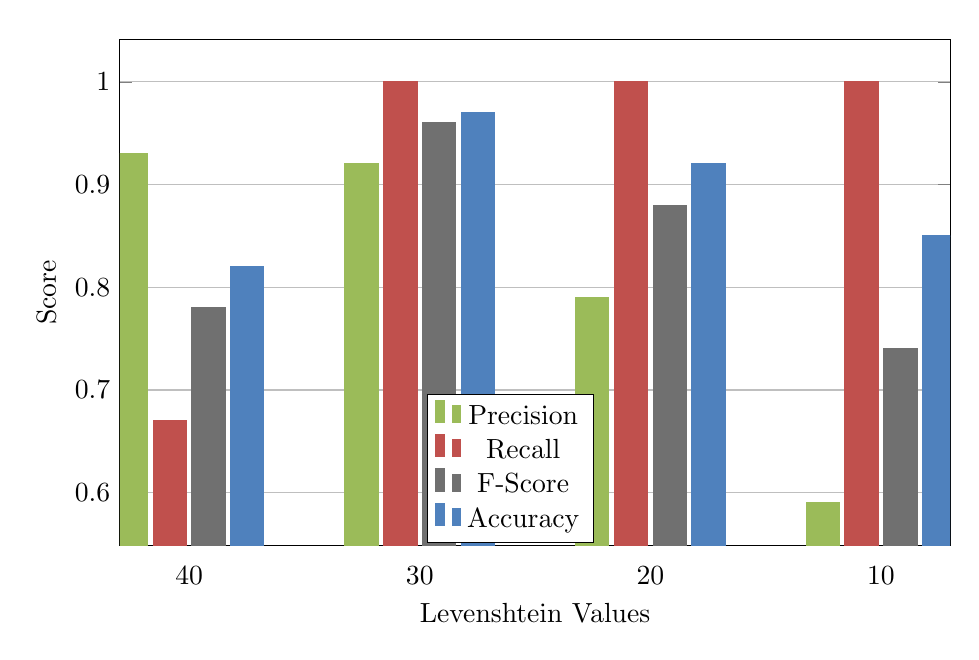
\begin{tikzpicture}
    \begin{axis}[
        width  = 1.00*\textwidth,
        height = 8cm,
legend style={at={(0.47,0.3)},anchor=north},
        major x tick style = transparent,
        ybar,
        bar width=12pt,
        ymajorgrids = true,
	xlabel={Levenshtein Values},
	ylabel = {Score},
        symbolic x coords={40,30, 20, 10},
        xtick = data,
        scaled y ticks = false,
    ]


       \addplot[style={ggreen,fill=ggreen,mark=none}] % Precision
           coordinates {(40, .93) (30,.92)(20,.79)(10,.59)};

      \addplot[style={rred,fill=rred,mark=none}] % Recall
             coordinates {(40, .67) (30,1)(20,1)(10,1)};

     \addplot[style={ggrey,fill=ggrey,mark=none}] % F-Score
           coordinates {(40, .78) (30,.96)(20,.88)(10,.74)};

        \addplot[style={bblue,fill=bblue,mark=none}] % Accuracy
            coordinates {(40, .82) (30,.97)(20,.92)(10,.85)};


     \legend{Precision,Recall, F-Score, Accuracy}

    \end{axis}

\end{tikzpicture}



\end{tabular}
  \captionof{figure}{Levenshtein Impact In Control Environment}
\label{fig:levencontrol}
\end{center}


\begin{center}
\begin{tabular}{lp{4cm}}

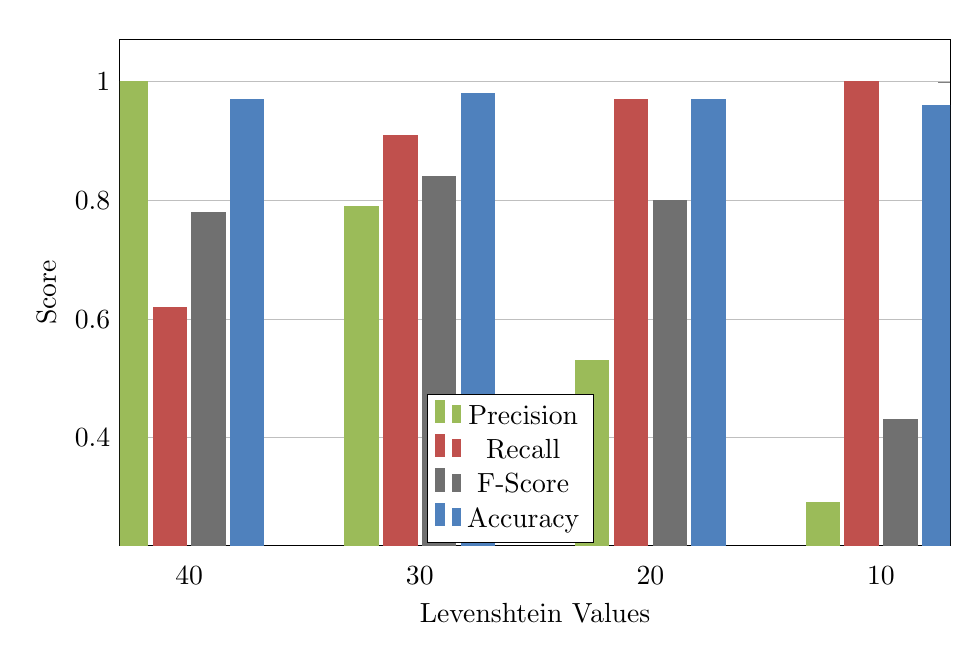
\begin{tikzpicture}
    \begin{axis}[
        width  = 1.0*\textwidth,
        height = 8cm,
legend style={at={(0.47,0.3)},anchor=north},
        major x tick style = transparent,
        ybar,
        bar width=12pt,
        ymajorgrids = true,
	xlabel={Levenshtein Values},
	ylabel = {Score},
        symbolic x coords={40,30, 20, 10},
        xtick = data,
        scaled y ticks = false,
    ]

       \addplot[style={ggreen,fill=ggreen,mark=none}] % Precision
           coordinates {(40, 1) (30,.79)(20,.53)(10,.29)};

        \addplot[style={rred,fill=rred,mark=none}] % Recall
             coordinates {(40, .62) (30,.91)(20,.97)(10,1)};


   \addplot[style={ggrey,fill=ggrey,mark=none}] %F-Score
           coordinates {(40, .78) (30,.84)(20,.8)(10,.43)};

             \addplot[style={bblue,fill=bblue,mark=none}] % Accuracy
            coordinates {(40, .97) (30,.98)(20,.97)(10,.96)};

     \legend{Precision,Recall, F-Score, Accuracy}


%\hspace{-1.3in}
    \end{axis}

\end{tikzpicture}

\end{tabular}
  \captionof{figure}{Levenshtein Impact In Open Source Applications}
%   \label{levencontrol}
\label{fig:levenopen}
\end{center}

%\begin{center}
%\begin{tabular}{lp{4cm}}

%\begin{tikzpicture}
  %  \begin{axis}[ybar stacked,
%	legend pos=outer north east,
%	reverse legend=true,
%	major x tick style = transparent,
%	major y tick style = transparent,
%	ymajorgrids = true,
%	xlabel={Levenshtein Values},
%	ylabel = {Score},
%	symbolic x coords={40,35,30, 25, 20, 15, 10}]

   %    \addplot[style={ggreen,mark=none,pattern=north east lines,pattern color=ggreen}] % Precision
    %       coordinates {(40, .93) (35,.93) (30,.92)(25,.87)(20,.79)(15,.77)(10,.59)};

    %  \addplot[style={rred,mark=none,pattern=vertical lines,pattern color=rred}] % Recall
     %        coordinates {(40, .67) (35,.97) (30,1)(25,1)(20,1)(15,1)(10,1)};

   %  \addplot[style={ggrey,fill=ggrey,mark=none,pattern=north west lines,pattern color=ggrey}] % F-Score
%           coordinates {(40, .78) (35,.95) (30,.96)(25,.94)(20,.88)(15,.87)(10,.74)};

  %      \addplot[style={bblue,mark=none,pattern=horizontal lines,pattern color=bblue}] % Accuracy
    %        coordinates {(40, .82) (35,.96) (30,.97)(25,.96)(20,.92)(15,.92)(10,.85)};


   %  \legend{Precision,Recall, F-Score, Accuracy}

%    \end{axis}

%\end{tikzpicture}
%\end{tabular}
%  \captionof{figure}{Levenshtein Impact In Control Environment - Stacked Bar Chart}
%\label{fig:levencontrol}
%\end{center}


%\begin{center}
%\begin{tabular}{lp{4cm}}

%\begin{tikzpicture}
 %   \begin{axis}[ybar stacked,
%	legend pos=outer north east,
%	reverse legend=true,
%	major x tick style = transparent,
%	major y tick style = transparent,
%	ymajorgrids = true,
%	xlabel={Levenshtein Values},
%	ylabel = {Score},
%	symbolic x coords={40,35,30, 25, 20, 15, 10}]

   %    \addplot[style={ggreen,mark=none,pattern=north east lines,pattern color=ggreen}] % Precision
   %        coordinates {(40, 1) (35,.92) (30,.79)(25,.64)(20,.53)(15,.35)(10,.29)};

   %     \addplot[style={rred,mark=none,pattern=vertical lines,pattern color=rred}] % Recall
     %        coordinates {(40, .62) (35,.78) (30,.91)(25,.93)(20,.97)(15,1)(10,1)};


  % \addplot[style={ggrey,fill=ggrey,mark=none,pattern=north west lines,pattern color=ggrey}] %F-Score
   %        coordinates {(40, .78) (35,.85) (30,.84)(25,.76)(20,.8)(15,.52)(10,.43)};

      %       \addplot[style={bblue,mark=none,pattern=horizontal lines,pattern color=bblue}] % Accuracy
       %     coordinates {(40, .97) (35,.98) (30,.98)(25,.98)(20,.97)(15,.97)(10,.96)};

   %  \legend{Precision,Recall, F-Score, Accuracy}


%%\hspace{-1.3in}
  %  \end{axis}
%\end{tikzpicture}
%\end{tabular}
 % \captionof{figure}{Levenshtein Impact In Open Source Applications - Stacked Bar Chart}
%%   \label{levencontrol}
%\label{fig:levenopen}
%\end{center}

%\sam{Stacked bar chart done - grayscale compatible.  Approve and delete originals.  I wonder if we shouldn't add data points at 45 and possibly 50}

In the controlled environment with the clones from Krawitz and Roy~\emph{et al.}, accuracy, recall, and precision values were collectively highest when a Levenshtein score of 30 was used. Similar results were observed when analyzing the open source applications for clones. A higher Levenshtein score is likely to discover more clones, but will also lead to more false positives, creating high precision but lower recall. Conversely, a low Levenshtein score will find fewer actual clones, but also have less false positives leading to high recall, but low precision. This is because a higher Levenshtein score means that the similarity threshold for noting cloned items will be reduced. A user could select different Levenshtein values depending on their desired levels of precision, recall, F-Score and accuracy.

These findings are important for several reasons. In both examples, the most appropriate Levenshtein score for attaining the highest accuracy, recall and precision was found to be 30, and this value has been used throughout our analysis. Additionally, these findings are indicative of those that future researchers may expect when using concolic analysis to find clones in their respective applications. In certain situations, researchers may wish to increase the recall or precision of their clone discovery technique, using resulting data to seek the most appropriate values.


\subsection{Calculated Levenshtein Distance \& Clone Types}

An interesting discovery is how calculated Levenshtein distance may show indication of clone type. In general, a lower calculated distance score is indicative of a closer level of similarity between two compared items. Overall, the average similarity score for all types of clones was 21.77, while non-clones averaged 71.19. A smaller variation would likely lead to many more errors in the clone detection process. What is most interesting is that the average Levenshtein score between two compared methods may not only indicate if they are clones, but also may help to indicate what type of clone they are as well. These values were calculated by recording the Levenshtein distance for each type of identified clone in the oracle, along with items which were not clones. The scores were then averaged together; type-1 clones were found to have the lowest average, with more complicated clones showing progressively higher values. Final results are displayed in Figure~\ref{fig:levenclonetype}.


\begin{center}
\begin{tabular}{lp{4cm}}

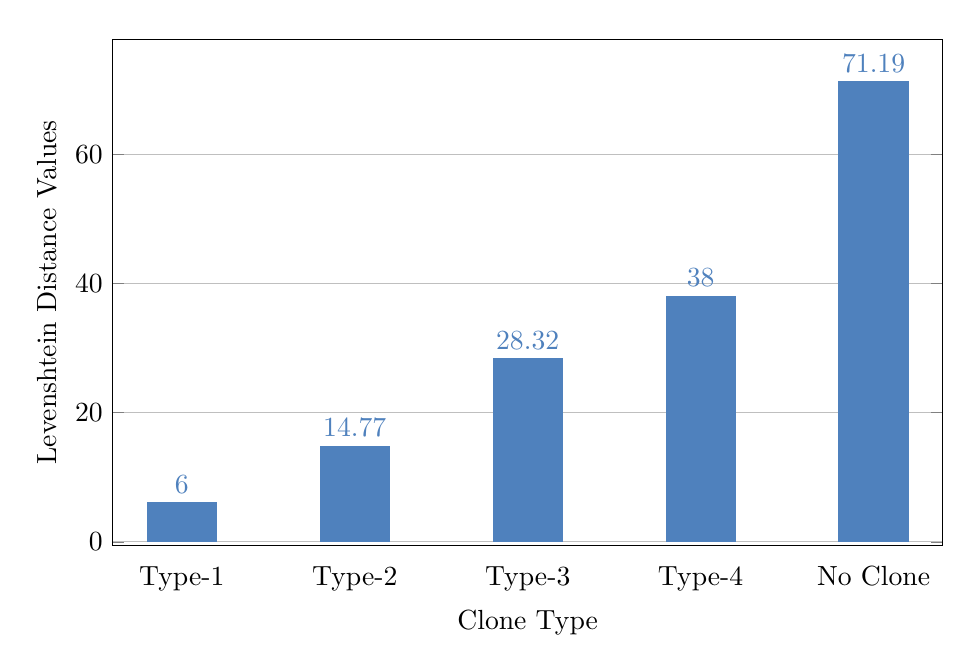
\begin{tikzpicture}
    \begin{axis}[
        width  = 1.0*\textwidth,
        height = 8cm,
        major x tick style = transparent,
        ybar,
        bar width=25pt,
        ymajorgrids = true,
	xlabel={Clone Type},
	ylabel = {Levenshtein Distance Values},
        symbolic x coords={Type-1, Type-2, Type-3, Type-4, No Clone},
        xtick = data,
        nodes near coords,
        scaled y ticks = false,
    ]

         \addplot[style={bblue,fill=bblue,mark=none}]
            coordinates {(Type-1, 6.00) (Type-2,14.77) (Type-3,28.32)(Type-4,38.00)(No Clone,71.19)};

   %     \legend{Accuracy,Recall,Precision}

%\hspace{-1.3in}
    \end{axis}

\end{tikzpicture}

\end{tabular}
  \captionof{figure}{Levenshtein Impact on Clone Types}
\label{fig:levenclonetype}
\end{center}

\section{Related Works}
\label{sec: relatedworks}
\todo{Beef up the related works section}

%	Talk about some of the other oracles out there that we did not used


There are numerous clone detection tools which utilize a variety of methods for discovering clones including text, lexical, semantic, symbolic and behavioral based approaches \cite{Roy:2009:CEC:1530898.1531101}. Only two , however, are known to be able to reliably detect type-4 clones.

MeCC discovers clones based on the ability to compare a program's abstract memory states. While this work was successful in finding type-4 clones, there are several areas for improvement such as its limitation in analyzing pre-processed C programs and an excessive clone detection time, likely caused by the exploration of an unreasonably large number of possible program paths~\cite{Kim:2011:MMC:1985793.1985835}. Krawitz~\cite{Kraw2012} proposed a clone discovery technique based on functional analysis which was shown to detect clones of all types, but was never implemented into a reasonably functional tool. This technique also requires a substantial amount of random data, which may be a difficult and time consuming process to produce.

CCFinder is a powerful clone detection tool which has been extensively referenced in existing clone detection research~\cite{Kamiya:2001:MST:381473.381749,Choi:2011:ECC:1985404.1985407,Hotta:2010:DCM:1862372.1862390}. The process used first transforms the input source text and then performs a token-by-token comparison in order to discover clones~\cite{Kamiya:2002:CMT:636188.636191}. While this tool has been evaluated in a significant amount of previous research, all links to download the application from its website appear to be dead, so it was unable to be evaluated in our work.\dan{Updated this sentence}

The most prominent area that concolic analysis has been applied to thus far is software testing, specifically for dynamic test input generation, test case generation, and bug detection \cite{Wassermann:2008:DTI:1390630.1390661, Sen:2005:CCU:1081706.1081750, Kim:2012:IAC:2337223.2337373}. Several tools exist for performing concolic analysis, including Crest \footnote{http://code.google.com/p/crest/}, Java Path Finder \footnote{http://babelfish.arc.nasa.gov/trac/jpf/}, CUTE \cite{Sen:2005:CCU:1081706.1081750}, and Pex \footnote{http://research.microsoft.com/en-us/projects/pex/}.

Tempero~\cite{IWSC13p53} described a collection of 1.3M method-level-clone-pairs from 109 different systems. The goal of this work was to create a similar data set for clone research. While this work was profound, much of the data has a low level of confidence and requires further work and analysis. Additionally, the clones are only from Java-based systems.

Lavoie and Merlo~\cite{Lavoie:2011:ATC:1985404.1985411} created an clone oracle set containing type-3 clones using the Levensthein metric. There was no mention of type-4 clones being created as part of this oracle, and the provided oracle only contained Java code. Krawitz~\cite{Kraw2012} and Roy~\emph{et al.}~\cite{Roy:2009:CEC:1530898.1531101} both defined clones of all four types in a small controlled environment. However, these works only specified a small number of clones which were artificially created.

\section{Threats to validity}
\label{sec: threats}


There are certain threats to the validity of our results. First, our results were only run on Java and C. We do not believe the results would significantly differ if concolic clone detection was run in different languages, but without verification it is impossible to tell for certain. Concolic analysis only executes the functional aspects of an application, meaning that it will not be able to detect clones in non-functional portions of the software. Second, this technique is limited by the concolic analysis tools available for use, and while these tools continue to improve and are robust, they are not perfect. In some cases they are unable to traverse various portions of an application or are incapable of recognizing segments of the application for technical reasons. This inhibits the clone detection process for these portions of the application. Finally, the followed path conditions depend upon the control flow graph and its predicates, meaning that concolic analysis for clone detection is still dependent upon its implementation. While it is less dependent than syntax or token based clone detectors, many code instances of identical semantics or different implementations will not be detected by concolic analysis for clone detection.

A significant portion of this study was based off previous research by Krawitz~\cite{Kraw2012}, Roy~\emph{et al.}~\cite{Roy:2009:CEC:1530898.1531101} and Kim~\emph{et al.}~\cite{Kim:2011:MMC:1985793.1985835}. Therefore, our results depend to a certain extent on the benchmarks provided by the aforementioned prior work. Manually finding type-4 clones in source code is extremely difficult and there is only one existing method known to reliably find type-4 clones. This makes it very difficult to test out a new mechanism in finding these clones specifically because there are very few benchmarks to be evaluated against. We are confident that concolic analysis is able to discover type-4 clones as is exemplified by our evaluation using the small sample oracle largely derived from Krawitz~\cite{Kraw2012} and Roy~\emph{et al.}~\cite{Roy:2009:CEC:1530898.1531101}. Unfortunately, since type-4 clones are very hard to manually identify and are only found by one existing tool, generating an accurate evaluation of a new technique in its ability to accurately identify type-4 clones is very difficult.

While we did our best to manually identify and classify clones using several people, and previous research has demonstrated the difficulty and problems with manually identifying and classifying code clones~\cite{Walenstein:2003:PCT:950792.951349}. This indicates that other researchers may disagree with many of the clones identified and how they were classified in our work. This is a problem which is not at all unique to our work and is one that hinders other research as well~\cite{Lavoie:2011:ATC:1985404.1985411}.

There are also numerous clone detection tools that detect clones in numerous different ways. While we were able to compare concolic analysis to several other leading detection processes, it is unreasonable to attempt to compare them to all known techniques. Many clone detection tools have adjustable inputs which may be altered to determine the size of the methods examined for clones, along with the similarity score needed to determine if two methods are defined as clones. While we did our best to use the most appropriate input settings for each tool, it is quite possible that more appropriate settings could have been selected to yield more accurate results. When we were unsure of the most appropriate setting, we chose to use the defaults for each tool.




\section{Future Work}



\dan{Show that concolic analysis COULD detect clones at the sub method level, but technique needs more pruning work}


\todo{Add in other work to be done}



\section{Conclusion}
\label{sec: conclusion}
\todo{Work on the conclusion}
In the future, we plan on applying the techniques described in this paper to other areas of computing research. One area we will research is how type-4 clones affect software development including how problematic they actually are. While existing research has examined many of the effects that simpler clones have on the software development lifecyle~\cite{Juergens:2009:CCM:1555001.1555062}, to our knowledge no work has been done to analyze the effect of type-4 clones specifically in that context.

Concolic analysis has only been evaluated in finding clones at the method level. However, many clones occur as only portions of methods, or across numerous methods. Future work is needed to determine the ability of the proposed technique in discovering clones at a more granular level or across methods.

Concolic Code Clone Detection represents a new and powerful clone detection technique. Concolic analysis executes various paths of an application. Similar application paths represents functional similarity, and thus a code clone candidate. When compared to leading existing clone detection tools, concolic analysis was able to more accurately and reliably identify all types of clones. The proposed clone detection technique is innovative because it not only represents the first known concolic-based clone detection technique, but is also one of only two known processes which are able to reliably detect type-4 clones.

%\vspace{5 mm}

\emph{Project Website:}
A complete implementation and more in depth results regarding this study may be found at the project website~\footnote{\url{http://www.se.rit.edu/~dkrutz/CCCD/}}

%~\cite{cccd_url}.

% Make sure the appendix goes after bib


%\bibliographystyle{spbasic}      % basic style, author-year citations
%\bibliographystyle{spmpsci}      % mathematics and physical sciences
%\bibliographystyle{spphys}       % APS-like style for physics
%\bibliography{}   % name your BibTeX data base
%\bibliographystyle{plain}
\bibliographystyle{spmpsci}
%\bibliographystyle{spbasic}      % basic style, author-year citations
\bibliography{refs}


\appendix
\section{Appendix}

We discussed precision, recall, F-score and accuracy in Section ~\ref{sec: acc_prec_rec}, where we omitted the results for several clone detection tools due to the inability to perform many of the calculations for specific tools since they were unable to find any clones. We present the complete results in Table~\ref{Table:Allprecisionrecall}, with incalculable values represented with an~\emph{x}.


\begin{table}[thb!]

\begin{center}
\caption{Precision, Recall, F-Score \& Accuracy for Each Tool}
\label{Table:Allprecisionrecall}
\begin{tabular}{r||l|l|l|l|l}
%  \hline
\bfseries Tool & \bfseries Source Example & \bfseries Precision & \bfseries Recall & \bfseries F-Score & \bfseries Accuracy \\ \hline\hline
  \bfseries Mecc-4 & \bfseries Control & 0 & x & x & .64  \\ \cline{2-6}
& \bfseries Apache & 1 & .3 & .46 & .88 \\ \cline{2-6}
& \bfseries P-SQL & 0 & 0 & x & .94 \\ \cline{2-6}
& \bfseries Python & 0 & 0 & x & .97 \\ \cline{2-6}
 \hline \hline
  \bfseries CloneDR & \bfseries Control & .78 & 1 & .88 & .67   \\ \cline{2-6} %CloneDR-80
& \bfseries Apache & 0 & x & x & .95 \\ \cline{2-6}
& \bfseries P-SQL & 0 & x & x & .95 \\ \cline{2-6}
& \bfseries Python & 0 & x & x & .97 \\ \cline{2-6}
 \hline \hline
  \bfseries Simian & \bfseries Control & .14 & 1 & .26 & .69   \\ \cline{2-6}
& \bfseries Apache & .06 & .33 & .1 & .94 \\ \cline{2-6}
& \bfseries P-SQL & 0 & x & x & .94 \\ \cline{2-6}
& \bfseries Python & 0 & x & ? & .97 \\ \cline{2-6}
 \hline \hline
  \bfseries Nicad & \bfseries Control & .59 & 1 & .74 & .85   \\ \cline{2-6}
& \bfseries Apache & .77 & 1 & .87 & .96 \\ \cline{2-6}
& \bfseries P-SQL & .03 & 1 & .06 & .95 \\ \cline{2-6}
& \bfseries Python & .67 & 1 & .8 & .97 \\ \cline{2-6}
 \hline \hline
  \bfseries CCCD & \bfseries Control & .92 & 1 & .96 & .97   \\ \cline{2-6}
& \bfseries Apache & 1 & .9 & .95 & .99 \\ \cline{2-6}
& \bfseries P-SQL & .73 & .96 & .83 & .98 \\ \cline{2-6}
& \bfseries Python & .67 & .84 & .75 & .98 \\ \cline{2-6}
 \hline %\hline

% \hline
\end{tabular}

\end{center}

%\vspace{-0.3in}
\end{table}

\end{document}
% end of file template.tex



%&&&&  Todo
% Add in references to MSR paper





% &&&&&&&&&&&&&&&&&&&&&&&&&&&&&&&&&&&&&&&&&&


%&&&& todo
% - check this format against the format from other works to this journal
% Bibliography is not correct
%       http://tex.stackexchange.com/questions/74634/problem-with-springer-bibliography-style  may be somewhat helpful

%- Make sure appendix is in the correct format
% I think the paper needs to be a bit wider. Compare it to other printouts of the same journal. % I think it is now ok. Check.
% Table names top or bottom? - Table top figures bottom
% Combine all multiple references

% Could not test against all. There are over X number of clone detection tools described in the works by X

% Describe the input parameters/options that were used for simcad
% Simcad does not mention type-4 clones in its options
% Mention the selection criteria for determining what were the "best" settings for each tool to get prec, recall etc....
% WIth the oracle, make sure that we state that the leven score was hidden during analysis. 